%
% Analysis and forecasting of the Swiss Rent Index
% 1993 to 2018
%
% authors:      Faralli Zully, Spörri Marc
% date-hand-in: 2018-05
%

\documentclass[11pt,a4paper]{article}

% Setup packages
% ------------------------------------------------------------------------

% set margins ect of page
\usepackage[
    a4paper,
    top=1in,
    bottom=1in,
    left=1in,
    right=1in
]{geometry}
% \usepackage{fullpage}  % don't use fullpage, use the more advanced geometry package

\usepackage[T1]{fontenc}
\usepackage[utf8]{inputenc} 

\usepackage[english]{babel}  % language settings
\usepackage{lmodern}         % font to use
\usepackage{chngcntr}        % to be able to change figure counters
\usepackage{makecell}        % make line breaks inside table cells
\usepackage{float}           % lets you place floats at a fixed place. DONT use it regulary!
\usepackage{placeins}        % lets you use floatbarriers

\usepackage{graphicx}        % use modern graphics formats

\usepackage{amsmath}         % math packages
\usepackage{amssymb}
\usepackage{siunitx}         % takes care of units and errors

\usepackage[round]{natbib}   % bibliography options

\usepackage{xcolor}          % use color names


% hyperref creates links in a pdf, and lets you set pdf options
\usepackage[
    pdfpagelabels,
    plainpages=false,
    pdfauthor={Faralli Zully, Spörri Marc},
    pdftitle={Analysis and forecasting of the Swiss Rent Index 1993 to 2018},
    pdfproducer={},
    pdfcreator={LaTeX2e (pdfLaTeX+Biber/Biblatex on Kile/TexLive/Debian9 and TeXnicCenter/MiKTeX2.9/Windows10)},
    pdfsubject={Analysis and forecasting of the Swiss Rent Index 1993 to 2018},
    pdfkeywords={swiss rent index}
]{hyperref}   % Hyperlinks

% clever refs lets you write just \cref{x} instead of figure~\ref{x}, section~\ref{y} ect..
\usepackage[
    %capitalise,   % cap the fig, table... refs
    noabbrev,     % use Figure instead of fig.
    nameinlink    % make the whole thing clickable
]{cleveref}


% Settings
% ------------------------------------------------------------------------

% fuer nicht eingerueckter Absatzbegin folgendes auskommentieren:
\setlength\parindent{0pt}    % laenge des absatzeinzuges festlegen

\counterwithin{figure}{section}  % include section number in figure numbering
\bibliographystyle{apa}      % bibliography style to use
\graphicspath{{graphics/}}   % all graphics are in the graphics folder.
                             % by default, search there!

% prevent empty pages with only one image by tweeking some parameters
\renewcommand{\topfraction}{.8}
\renewcommand{\floatpagefraction}{.8}  % if more than x % of a page is an image
                                       % it will be a single image page.
                             




% My own commands
% ------------------------------------------------------------------------

% note \TODO{} in teh sourcecode to get reminded later that you still have work todo
\newcommand{\TODO}[1]{%
    \textcolor{red}{ %
        \textbf{[ !!!TODO: #1 ]}%
    }%
    \PackageWarning{TODO:}{TODO: #1}%
}


% The actual document
% ------------------------------------------------------------------------
\begin{document}


% titlepage
% ------------------------------------------------------------------------
\pagenumbering{roman}
\thispagestyle{empty}  % no pagenumber on this page

\begin{center}

\vspace*{4cm}

\noindent\rule{15cm}{0.4pt}

\vspace*{2cm}

\Huge{\textbf{Analysis and Forecasting of the Swiss Rent Index, 1993 to 2018}}

\vspace{1cm}

\LARGE{Project in Time Series Analysis -- Spring 2018}

\vspace{2cm}

\noindent\rule{15cm}{0.4pt}

\vfill

\large{
    \today\\

}
\vspace{2cm}

%\large{Authors: Faralli Zully, Spörri Marc\\}
%\vspace{1cm}
\large{Institute of Statistics \\University of Neuchâtel}

\vspace{2cm}

\end{center}


\newpage



% TOC
% ------------------------------------------------------------------------
\thispagestyle{empty}
\tableofcontents

\newpage


% ------------------------------------------------------------------------
\pagenumbering{arabic}
\setcounter{page}{1}

\section{Introduction}

In this project we will analyse the time series of the quarterly collected Swiss rent index from 1993 to 2018.
The main goal of the project is to draw inference from the rent index time series and to predict its future values and a future trend.

In order to do that, first we transform the data into a mean-centered stationary time series by eliminating the trend and possible seasonal components.
Then, we model our transformed, stationary data by fitting and testing a set of auto-regressive moving average processes (ARMA) in order to select the best candidate model for our stationary data \cite[p.~82--110]{bd02}.
The selected model will be used to describe and interpret our data as well as to predict future values for the Swiss rent index.


% ------------------------------------------------------------------------

\section{Data Description and Data Analysis}

The data is provided by the Swiss Federal Statistical Office, implying 100 quarterly observations of the Swiss rent index beginning by Quarter 2, 1993 and ending by the Quarter 1, 2018.
The rent index measures the inflation of rented dwellings in Switzerland.
It is the most significant partial index of the Swiss Consumer Price Index, representing 13% of it.

\begin{figure}
    \centering
    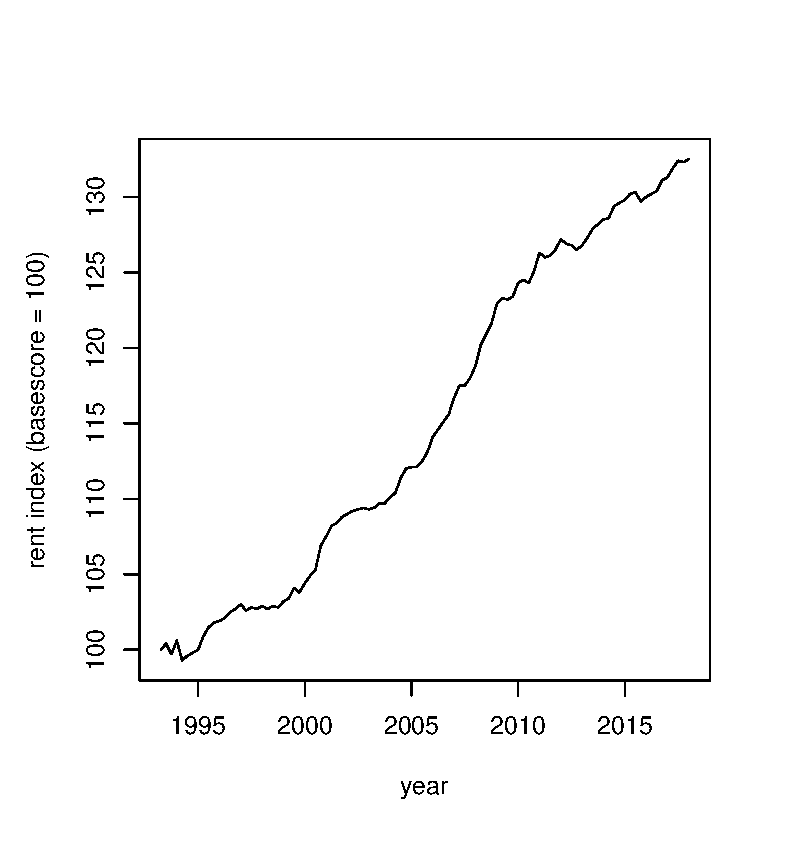
\includegraphics[width=0.7\textwidth]{indiceloyers_timeseries}
    \caption{Swiss rent index, years 1993 to 2018}
    \label{fig:indiceloyers_timeseries}
\end{figure}

The data are collected quarterly, based upon a stratified random survey sampling of around \num{10000} lessors.
The time series' first observation (Quater2, 1993) will be the reference value which is set to a base index of 100 and represents the weighted average rent at this time in Switzerland \cite[p.~20--23]{ofs}.

The first step in any analysis of a time series is to identify possible discontinuities or a sudden change of level in the series \cite[p.~23]{bd02}.
As indicated in \cref{fig:indiceloyers_timeseries} there an evident be a positive monotonic trend in the time series of the Swiss rent index.
However, the increase seems to be higher in the 1990ies and we can detect a slightly slower increase in the period of 2009 to 2018, indicating that during the years 1993 to 2009 the growth rate of rents increased faster than during the years after 2009.

This fact can be explained by the big real estate depression in the early 1990ies in Switzerland.
Therefore, the time series starting in 1993 starts from a relatively low initial level.
Given this low initial level and the better conjunctural perspectives, the growth rate was faster during the 1990ies \citep{fuw}, whereas from the year 2009 on, the growth rate slowed down.
This can be explained by the US subprime crises triggered in the year 2008, followed by a long-lasting global recession.

Therefore, there are apparently no outliers, sudden changes or major discontinuities.
Moreover, the differences are not large enough that further data adjustments or variance-stabilizing transformations like Box-Cox-transformations have to be done \citep{boxcox64}.
Consequently, we start our work in the next section by transforming our data into a stationary time series.


% ------------------------------------------------------------------------

\section{Transformation of the Data into a Stationary Time Series}

The purpose in this section is to produce a noise sequence with no apparent deviations from stationarity.
This means we want to transform our data in such a way that covariances between the observations do not depend on time, also that we obtain a zero mean expectation and constant variances \cite[pp.~14--23]{bd02}.

However, the objective is not to get a pure white-noise sequence with no dependence among the residuals neither.
Otherwise, we would be confronted with too much randomness in our stationary series so our prediction work would be simply done by estimating the mean of the white-noise, which is zero for all predictions $X_{n+1}$, $X_{n+2}$, $X_{n+3}$ etc. (in case of a mean-centered stationary series).

Hence, the objective is to obtain a stationary series with some few significant dependence among the residuals, so we can look for a more complex stationary time series model for the noise that accounts for the dependence.
Since dependence means that past observations of the noise sequence can assist in predicting future values this would allow us to get a better prediction quality than we could with a pure white noise sequence \cite[p.~35]{bd02}.

In order to get our noise sequence we have to eliminate any trend and/or seasonal components from our data.
In the next few subsections we will fit several models to get a stationary series.
We will check them first visually by plotting the autocorrelation-function (ACF) as well as the partial auto-correlation function (PACF) in order to ensure that we are not modelling a white-noise sequence on the one hand, and on the other hand to get an idea of the orders of p and q for a possible ARMA(p,q)-model \cite[pp.~83--110]{bd02}.

We will test our fitted models for stationarity with the Augmented Dickie-Fuller-Test against the null hypothesis of a unit root (with the alternative hypothesis of stationarity, by consequence \citep{adf}).
In addition, we test the estimated noise sequences with the Ljung-Box-Test which examines whether or not the obtained residuals are values of independent and identically distributed random variables (\citep{LjungBox78}).

Once we have found a good way to transform our data into a stationary series we will fit and test a set of candidate models for our transformed data in \cref{sec:FitTestModel}.



\subsection{Method 1: Trend Elimination by fitting polynomial models}

Since the time series in figure \ref{fig:indiceloyers_timeseries} let us suggest a probable polynomial trend, especially a linear one, we start by fitting different polynomial trends by ordinary least squares estimation \cite[p.~11]{htf09}.

Now we model a noise sequence (residual time series) by estimating and subtracting a linear, a quadratic, a cubic as well as a logarithmic trend.
The latter  helps to transform a potentially exponential increase in the rent index into a linear trend, even though our time series (\cref{fig:indiceloyers_timeseries}) looks more like a linear than an exponential trend at first glance, we are going also to test for a logarithmic trend.

The regression models by ordinary least squares estimation \cite[p.~11]{htf09} showed highly significant trend coefficients for all four polynomial models and no significant seasonal effects have been detected.\footnote{
    Since the data are collected quarterly we used a linear regression model with d=4 dummy predictors to check for significant seasonal coefficients, meaning a dummy for every quarter (see \cref{sec:summarystat}).
}


Thus, all of the polynomial models would explain our data extremely well which is indeed not surprising, given the fact that the trend is consistently positively monotonic and therefore highly consistent with other positively monotonic models as our four polynomial trend models indeed are (further details on the estimated trend coefficients and seasonal coefficients as well as the corresponding significance levels can be found in \cref{sec:summarystat}).\footnote{
    Interpretation of p-values of regression model coefficients are to be handled with care in the case of time series.
    This because these models are assuming independence of the observations which hardly never holds true in a time series except white-noise.
    We have to keep in mind that in case of time series we don't want to draw inference on the regression coefficients, our purpose for the regression coefficients is a different one: by looking at their p-value we get an idea whether or not there is a polynomial trend to eliminate in order to get a stationary time series
}


Nevertheless, even though there is evidently a highly significant polynomial trend in the Swiss rent index series, this does not mean necessarily that its residual time series are stationary.
Unfortunately, this happens to our four noise sequences, as illustrated in \cref{fig:resid_polynomials}.
\begin{figure}
    \centering
    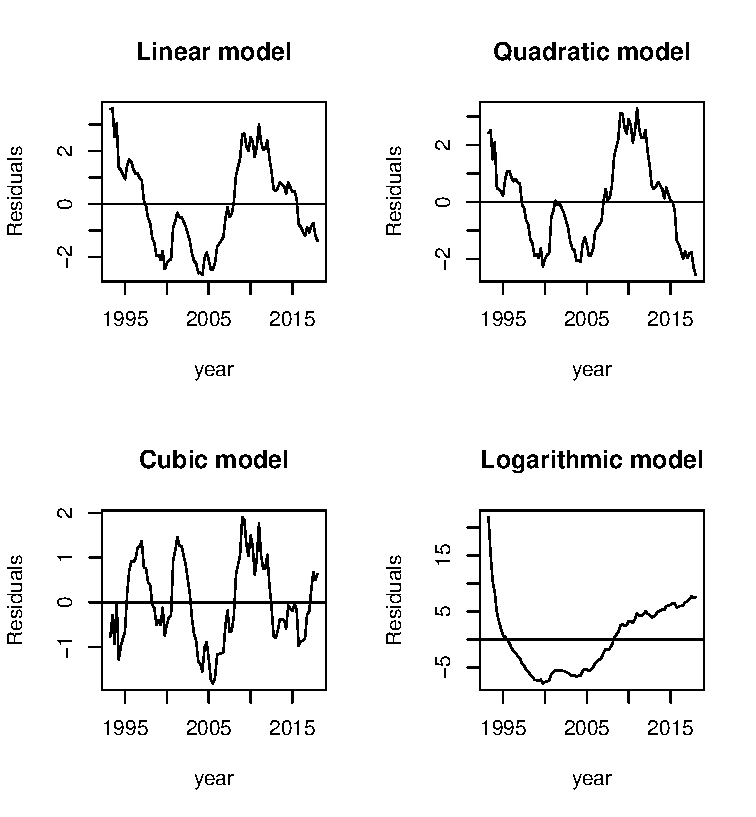
\includegraphics[width=0.7\textwidth]{resid_polynomials}
    \caption{Residuals of the fitted linear, quadratic, cubic and logarithmic model}
    \label{fig:resid_polynomials}
\end{figure}

The series wander up and down for quite some periods, which means that the basic properties of stationary processes, time-independent expectation and constant variance over time are not fulfilled here \cite[p.~49]{bd02}.
Since we can already be sure thanks to the residual plots, that trend elimination by fitting polynomial models does not help to obtain a stationary series, we will not show further diagnostics on these and continue by trying to eliminate the trend by differencing.\footnote{
    Since the residual plots show strong time-depending covariances, by consequence the plots of the sample auto-correlation function (ACF) and partial auto-correlation function (PACF) of the fitted polynomial models showed likewise a strong auto-regressive process of order 1 (decreasing values in the ACF-plot and 1 spike in the PACF-plot with a lot of significant auto-correlations outside the 95-percent-confidence bounds of $\pm 1.96/\sqrt{n}$, see \cref{sec:acfpacfunused}).
}


\subsection{Method 2: Trend elimination by differencing}
Since the fitted polynomial models did not help to get a stationary time series, we will try to eliminate the trend by differencing.
We will now differentiate the data at different lags (1, 2, 3 and 4) in order to generate a noise sequence and get a stationary series \citep[p.~35]{bd02}.
Again, we will show first the residual plots.
Afterwards, testing will be done by looking at the sample ACF and PACF as well as the Ljung-Box-Test for indepencence of the residuals and the Augmented Dickie-Fuller-Test for stationarity.


\subsubsection{Modelling the estimated noise sequences}

\begin{figure}
    \centering
    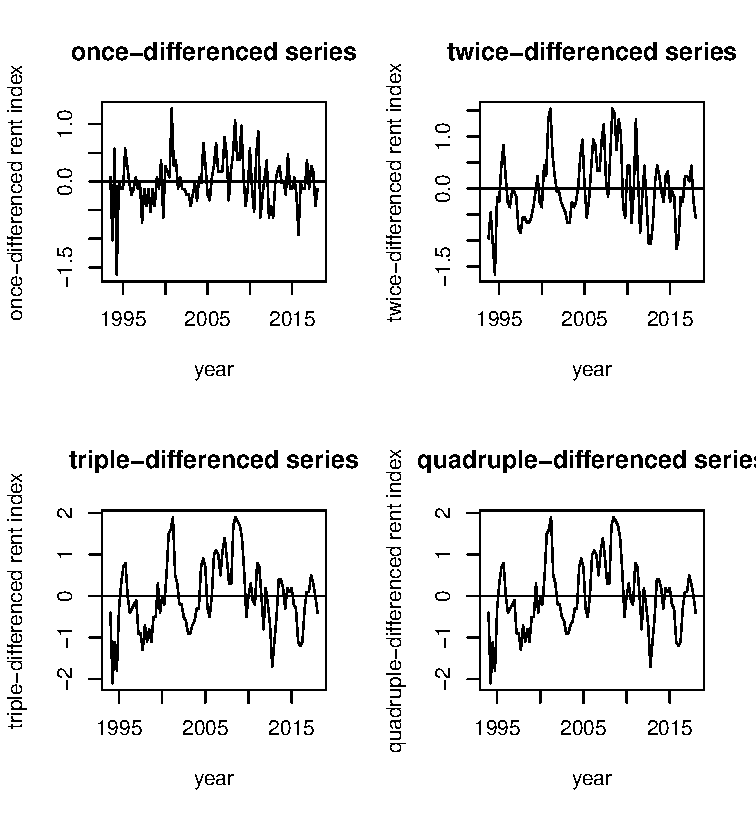
\includegraphics[width=0.7\textwidth]{resid_diff_all}
    \caption{Residuals of the differenced series}
    \label{fig:resid_diff_all}
\end{figure}

As indicated in the \cref{fig:resid_diff_all} the first two models look already quite promising in contrast to the polynomial models above, showing here obviously time-independent noise sequences with presumably constant variance.

The lag1-differenced series show mostly patterns of a white-noise which is not what we want since, a white-noise induces too much randomness and the prediction quality would become rather poor.


\subsubsection{Testing the noise sequences}

First, we are going to test the estimated trends visually, by looking at the sample ACF and PACF.
Then, we will apply the diagnostic tests for white-noise (Ljung-Box-Test (\citep{LjungBox78}) and for stationarity (Augmented Dickie-Fuller-Test for stationarity (\citep{adf})), respectively:

As we can see in \cref{fig:diff12_acf_pacf}) the white-noise of the lag1-differenced series is confirmed by the sample ACF where all lags up to 40 fall within the bounds of $\pm 1.96/\sqrt{n}$ \cite[p.~39]{bd02}.
This emphasizes the suggestion that the lag1-differenced series is too versatile and contains too much randomness.

\begin{figure}
    \centering
    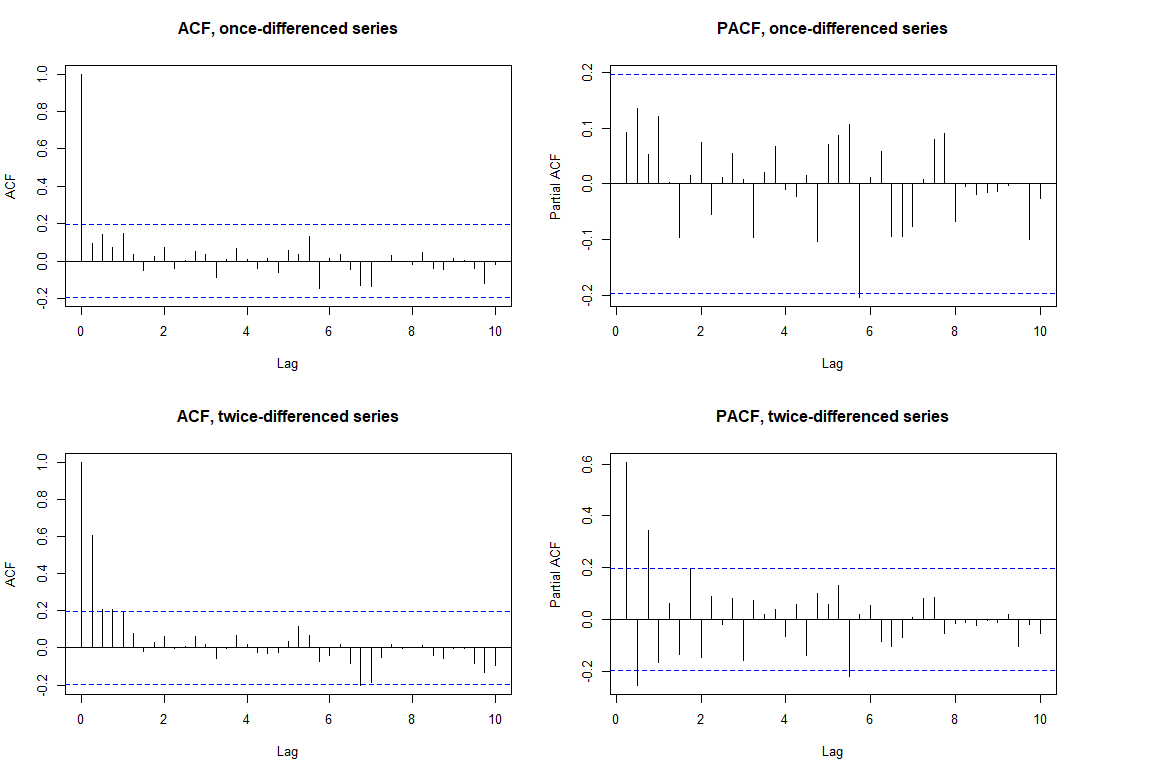
\includegraphics[width=0.9\textwidth]{diff12_acf_pacf}
    \caption{Sample auto-correlation and partial auto-correlation function of the lag1- and lag2- differenced series}
    \label{fig:diff12_acf_pacf}
\end{figure}

In contrast, the sample ACF of the lag2-differenced model does not indicate a white-noise: we can see at least one highly significant auto-correlation at lag1 and the following three bars touching the 95 percent-confidence-bounds of $\pm 1.96/\sqrt{n}$, followed by no more significant bars which die out quickly.
This is a good sign, because on one hand, we have at least correlation at lag 1 which is needed to do prediction and, on the other hand, the covariances seem obviously not time-dependent and therefore we can suggest a stationary series here.

\begin{table}
\centering
\begin{tabular}{c|cccc}
    Differentiation at:  & lag1 & lag2 & lag3 & lag4 \\
    \hline 
    \makecell{p-value Ljung-Box-Test\\($H_0$: White-noise)} & 0.35 & 0.00 & 0.00 & 0.00\\
    \makecell{p-value Augmented Dickie-Fuller-Test\\($H_0$: Non-Stationarity)} & 0.01 & 0.05 & 0.11 & 0.42\\
\end{tabular}
\caption{Overview of the diagnostic tests for the differenced series}
\label{table:overview_diffs}
\end{table}

From the test's overview in \cref{table:overview_diffs} we can see for the lag1-differenced series a p-value of 0.35 for the Ljung-Box-Test.
That was expected and means that we cannot reject the hypothesis $H_0$ which assumes that there is independence between the observations \citep{LjungBox78} and therefore confirming the white-noise structure in the lag1-differenced series.

In contrast again, the Ljung-Box-Test for the lag2-differenced series rejects the $H_0$ of independence which is a pleasant result giving us the sureness that there is no white-noise in the lag2-differenced series.
The Augmented Dickie-Fuller-Test suggests a stationary time series for the lag1- as well as for the lag2-differenced trend elimination (p-values < 0.05).

That is a promising result and we can finally conclude to stick with the lag2-differentiation since the lag1-differenced series is characterized by too much randomness.
Also because white-noise and the lag3- and lag4-differenced series show too large covariances (time-dependence/non-stationarity, indicated by high p-values of the Augmented Dickie-Fuller-Test by 0.11 and 0.42, respectively.
To conclude the transformation step we center our transformed data by subtracting the mean which is necessary to fit ARMA-models.


% ------------------------------------------------------------------------

\section{Fitting and Testing Models}
\label{sec:FitTestModel}

\subsection{Selection of order and models}

From the sample ACF and PACF (\cref{fig:diff12_acf_pacf}) of our lag2-differenced series, we saw in the ACF-plot one highly significant spike at the first auto-correlation $\hat{\rho_1}$ and the following bars dying out quickly, lying inside the $+/-1.96/sqrt{n}$ - bounds.
Thus, the single spike in the ACF-plot together with the exponentially decreasing patterns in the PACF-plot let us suggest an MA(1)-model could fit well our data.

However, since we are operating with only 100 observations, we cannot be sure that there are not underlying exponentially decreasing patterns in the ACF plot.
This also because the bars die out so quickly.
If this would be the case, then an exponential decrease (in absolute values) in both the ACF and PACF plot would rather suggest an ARMA-model.


Hence, we follow a conservative approach and compare the AICC-value of the MA(1) as well as AICC-values\footnote{
    The lower the AICC-value the better the model's performance \citep{aic86}.
}
for ARMA-models with different orders of p and q\footnote{
    p indicates the order of the auto-regressive part and q the order of the moving-average part.
    Its coefficients are generally noted as $phi$ (AR-part) and $theta$ (MA-part).
} 
in order to select our model (for further details on all possible AICC-values up to $p=5$ and $q=5$, see the AICC-matrix \cref{fig:aicc_matrix} and \cref{sec:aicc_matrix}).

The MA(1)-model gives us the lowest AICC-value which means this model is supposed to perform best.That confirms our presumption based on the sample ACF/PACF plots.
However, we will also fit an ARMA(1,1) and an ARMA(1,2) model, because both of them showed as well very low AICC-values (see AICC-Matrix in figure).\footnote{
    Estimations by the autofit-function of the "itsmr" package of R by \citet{R_itsmr} suggest as well an MA(1)-model as best model with a very similar estimate for $\theta_1$ and very close AICC.
    Furthermore ARMA(1,1) and ARMA(1,2) are also suggested by the autofit()-function showing very low AICC-values.
    This can be seen as a successful robustness check in terms of order selection of p and q.
}

We will now estimate coefficients for these three model candidates by the arima-function of the R-package "stats" (\citet{R_stats}).\footnote{In brackets standard errors of the estimated coefficients.}
\begin{align*}
    \text{MA(1)-model:} \quad & X_t = Z_t + \theta_1 Z_{t-1} \\
    & \text{where:} \  {Z_t} \sim WN(0,\sigma^2)  \\
    & \text{with:} \ 
        \hat{\theta}_1 = \num{ 1.00 \pm 0.07}, \ 
        \hat{\sigma}^2 = \num{ 0.18 }
\\
    \text{ARMA(1,1)-model:} \quad & X_t - \phi_1 X_{t-1} = Z_t + \theta_1 Z_{t-1} \\
    & \text{where:} \  {Z_t} \sim WN(0,\sigma^2) \\
    & \text{with:} \ 
        \hat{\phi}_1 = \num{ 0.13 \pm 0.11}, \ 
        \hat{\theta}_1 = \num{ 0.98 \pm 0.08}, \ 
        \hat{\sigma}^2 = \num{ 0.18 }
\\
    \text{ARMA(1,2)-model:} \quad & X_t - \phi_1 X_{t-1} = Z_t + \theta_1 Z_{t-1} + \theta_2 Z_{t-2} \\
    & \text{where:} \  {Z_t} \sim WN(0,\sigma^2) \\
    & \text{and:} \ 
        \hat{\phi}_1 = \num{ 0.80 \pm 0.21}, \ 
        \hat{\theta}_1 = \num{ 0.31 \pm 0.25}, \ 
        \hat{\theta}_2 = \num{-0.67 \pm 0.26}, \ 
        \hat{\sigma}^2 = \num{0.18}
\end{align*}

First we can see that an ARMA(1,1)-model is not supposed to be a good model.
Its estimated coefficient $\hat{\phi}_1=0.13$ is not significant, since its standard error of 0.11 is nearly as high as the coefficient.

In contrast, an ARMA(1,2)-model looks quite promising.
First, its AR-term is significant, taking a value of $\hat{\phi}_1=0.80$ and second, we can provide evidence for the estimates of the two MA-terms by considering an additional MA-term.
Then, the ARMA(1,3)'s coefficients $\hat{\theta}_1 = 0.35$ and $\hat{\theta}_2= -0.60$ would not differ a lot from the ARMA(1,2)'s coefficients $\hat{\theta}_1 = 0.31$ and $\hat{\theta}_2 = -0.67$.
Furthermore, the additional MA-term $\hat{\theta}_3 = 0.05$ in the ARMA(1,3) model is not significant since it would be close to zero with a large standard error, indicating that the explanatory power by adding a third $\hat{\theta}$- term would be rather poor.
Therefore, the comparison with the overfitted ARMA(1,3) confirms that a moving-average of order 2 would be a suitable choice.
But, we have to note that $\hat{\theta}_1$ and $\hat{\theta}_2$ in the ARMA(1,2) model are rather small compared to their standard errors.
$\hat{\theta}_1$ is only slightly larger than its standard deviation.
$\hat{\theta}_2$ is 2.5 times larger.

The MA(1) is also performing very well, but with a value of 1.00 for $\hat{\theta}_1$ there exists a unit root on the moving-average polynomial.
However, that is of minor importance compared to unit roots on the auto-regressive polynomial \cite[p.~42--83]{bd02} which would be severe because that would mean non-stationarity.
Fortunately it is not the case here.
Therefore we want to stick with the MA(1) and ARMA(1,2) as our candidate models.


\subsection{Diagnostics of the models}
To check the validity of our candidate models we will apply the following diagnostics:

First, we plot the rescaled residuals and check for randomness.
We expect a white-noise if the model is valid.
Second, we have a look at the ACF of the rescaled residuals.
Since we are supposed to have a white-noise, approximately 95 percent of the sample-autocorrelations $\hat{rho}$ should lie inside the bounds of $\pm 1.96/\sqrt{n}$.
Third, we use the Ljung-Box Test \citep{LjungBox78} to validate or not that the residuals are white-noise by showing the p-values for each lag \cite[Lecture~11]{chevalier18}.

\begin{figure}
    \centering
    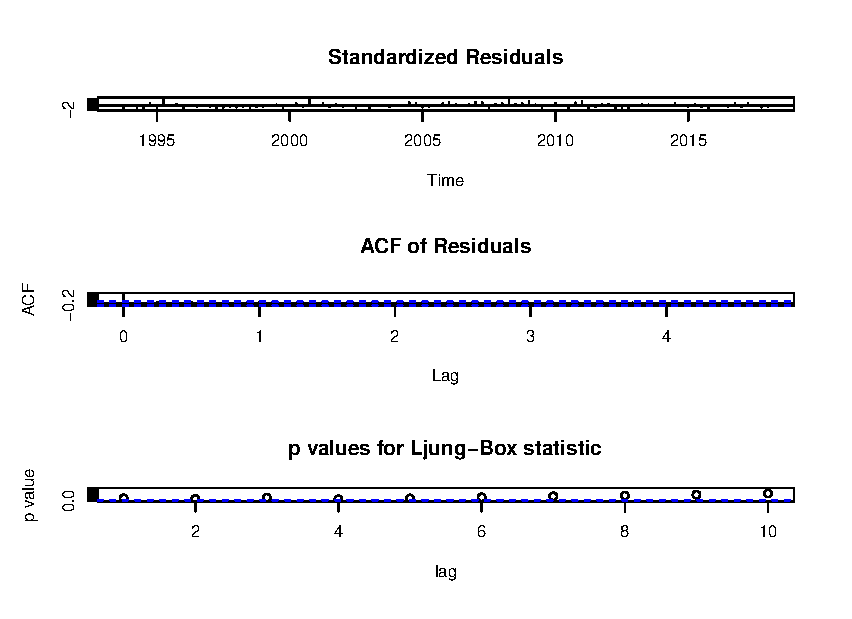
\includegraphics[width=1\textwidth]{ts_diag_ma_1}
    \caption{Standardized Residuals, Auto-correlation function of the Residuals and the p-values for the Ljung-Box-Test (left side: MA(1); right side ARMA(1,2)}
    \label{fig:ts_diag_ma_1}
\end{figure}


We visualize these diagnostics by using the tsdiag() function from the "stats" R-Package (\citet{R_stats}).
The following figures in \cref{fig:ts_diag_ma_1} illustrate these three results for both of our candidate models, the MA(1) on the left hand side and the ARMA(1,2) on the right hand side.
We can see that the standardized residuals are supposed to be white-noise in both cases.
In addition, from the ACF of the rescaled residuals we can see that none of the bars (out of 20) lies outside the bounds $\pm 1.96 / \sqrt{n}$ which indicates what we need: a white-noise.
Furthermore, from the Ljung-Box-Tests we can see that the p-values are larger than 5 percent for each lag in both cases MA(1) and ARMA(1,2), meaning we cannot reject the Hypothesis H0 which states that these residuals are white-noise.
Especially the ARMA(1,2) shows very large p-values and can therefore be considered to perform very stable in terms of white-noise.
As a consequence, both models MA(1) and ARMA(1,2) passed the tests and turn out to be valid models for forecasting.


% ------------------------------------------------------------------------

\section{Prediction of future values}

The purpose of this section is to predict future values on the base of our fitted MA(1)- and ARMA(1,2)-models.
First, we will do that by forecasting our transformed (lag2-differenced) series.
Afterwards we will forecast the initial time series and predict its future values.
95 percent confidence bands will be given in case of normally distributed residuals.

\begin{figure}
    \centering
    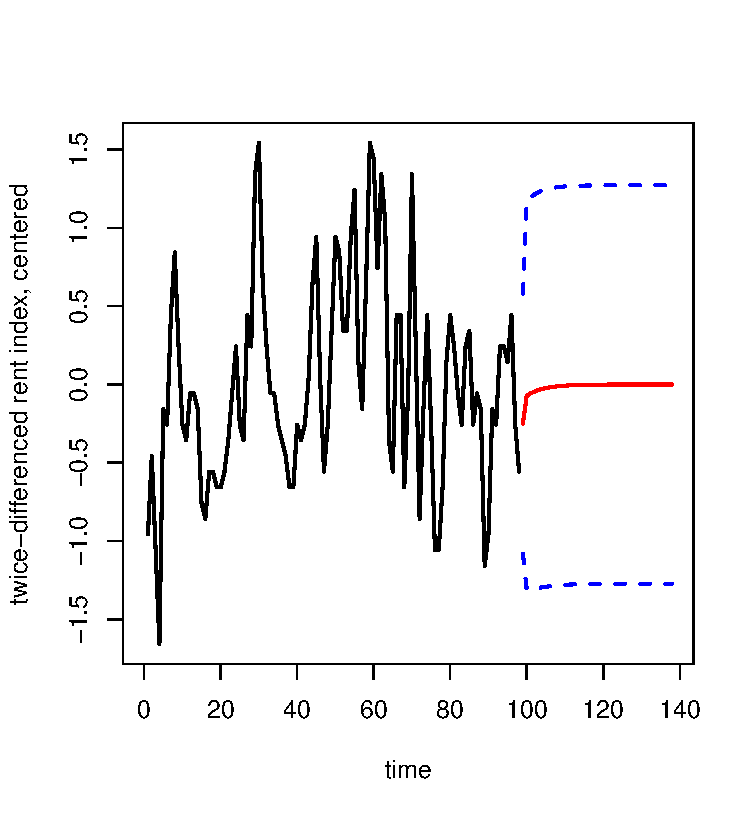
\includegraphics[width=0.6\textwidth]{pred_transformed_series}
    \caption{Prediction and confidence bands for the lag2-differenced Series, MA(1) and ARMA(1,2)}
    \label{fig:pred_transformed_series}
\end{figure}

\cref{fig:pred_transformed_series} illustrates the prediction of a process of adaptation to the zero-mean for the next 8 quarters.
Both models show a prediction tendency to the zero-mean which is nothing surprising for a mean-centered stationary time series.
However, the ARMA(1,2)-model predicts a smoother and slower convergence to the zero-mean as we can see from the red prediction line in the bottom plot, representing a more traceable and more realistic forecast.
In contrast, the MA(1)-model would only predict for $X_{n+1}$ a value different from the zero-mean.
For all the following $X_{n+2}$,$X_{n+3}$ etc. the MA(1)-model would abruptly predict a zero-mean, as we can see from the red prediction line in the top plot.
Hence, the MA(1)-model's prediction power is not that high and with exception of the prediction of $X_{n+1}$, would not even differ from predictions based on a pure white noise sequence.

The quite large 95-percent confidence bands (blue lines) are not that surprising in a differenced series.
Differenced series can contain quite large amplitudes as we can see from the past observations.\footnote{
    The indication of confidence bands is weakly justified here, since the series’ residuals are successfully tested for normal distribution by the Shapiro-Wilk-Normality-Test which gave us a p-value of 0.12 in case of MA(1) and 0.07 in case of ARMA(1,2), meaning that the hypothesis H0 of normal distribution can not be rejected \citep{shapiro}.
    Due to the relatively low p-values, interpretations of confidence bands are to be handled with care.
}
However, it would be desirable to reduce the variance and likewise the confidence bands by increasing the number of observations.
\begin{figure}
    \centering
    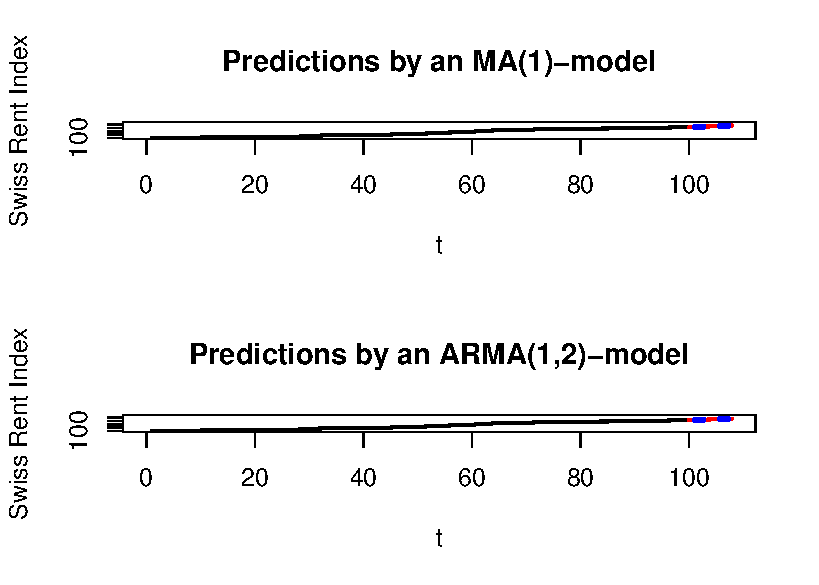
\includegraphics[width=0.6\textwidth]{pred_initial_series}
    \caption{Prediction and confidence Bands for the initial time series, MA(1) and ARMA(1,2)}
    \label{fig:pred_initial_series}
\end{figure}

The prediction of the initial series bases on retransformation of the lag2-differenced series into the initial series by the equations
\begin{align*}
    C_t &= \nabla_2 Y_t = Y_t - Y_{t-2}\\
    X_t &= C_t - \mu_{C_t} \\
    Y_{n+h} &= C_{n+h} + C_{n+h-1} + C_{n+h-2} + \ldots + C_{n+1} + Y_n  \\
    P_n Y_{n+h} &= h*\mu + Y_n+ P_n X_{n+1} + \ldots + P_n X_{n+h}
    \text{\ ,}
\end{align*}
where $Y_t$ is the initial time series series, $C_t$ the lag2-differenced series and $X_t$ is the mean-centered differenced series.
The $P_n Y_{n+h}$ represent the $h=8$ predicted future values for the initial time series, where $h*\mu$ represents the rate of the increase (slope) and the $P_n X_{n+1} + \ldots + P_n X_{n+h} $ are obtained by the MA(1)- and ARMA(1,2)-model, respectively.

In \cref{fig:pred_initial_series} we can see that the predictions for the initial time series are reasonable for both models MA(1) and ARMA(1,2), indicating a strongly monotonic trend in the future.
However, due to the smoother and slower convergence to the mean, we definitely want to stick with the more traceable and more realistic ARMA(1,2)-model as our favourite model.




% ------------------------------------------------------------------------

\section{Discussion}
The strength of the project lies in the forecast by the ARMA(1,2)-model which gives us a reasonable monotonically increasing prediction which smoothly adapts to the expected mean within the upcoming few quarters.
In contrast, the difficulty of this project was to transform the data into a stationary time series in a way that the residuals, on one hand, don't show too much randomness (no white-noise) and, on the other hand, we get a few significant auto-correlations $\hat{rho}$ in order to be able to forecast based upon past observations.
That turned out to be a challenging task because, first, trend elimination by polynomial trend fitting was not possible because of the heavy time-depending auto-covariances.
Second, linked to the trend elimination by differentiation we were confronted with the dilemma between a lag1-differentiation which would have led to an undesirable white-noise sequence and a lag4-differentiation which was not stationary any more (p-value of augmented Dickie-Fuller-Test of 0.42.
\footnote{
    The alternative hypothesis $H_A$ means stationarity \citep{adf}.
}
In between those two extreme options only the lag2-differentiation was stationary and allowed for better prediction quality on the same time, thanks to one significant auto-correlation $\hat{rho_1}$.
Nevertheless, even the lag2-differentiation is not a totally satisfying transformation since a lag2-differentiation is normally used to get rid of a two-periodical seasonal effect and our series was definitely not seasonal as proven in section 3 (for further details on the absence of seasonality see \cref{sec:summarystat}).
 
In addition, the MA(1)-model turned out to show a minor issue due to a unit root in the moving-average polynomial (estimated $\hat{\theta_1} = 1.00$) which could possibly indicate an overdifferencing according to \cite[~p.194]{bd02}.
When a root of the process is close to the unit circle the asymptotic distribution of the maximum likelihood can be quite inadequate \citep{davidson81}.
However, other authors have shown that an estimation by maximum likelihood differ only slightly from estimations by other methods (\citep{davisdunsmuir96} ).
A $\hat{\theta_1}$ close to 1 is therefore not that big of a deal and it is certainly from negligible importance in contrast to a unit root on the autoregressive polynomial \citep{plosser77}.

Furthermore, our model of choice, the ARMA(1,2) process, does in fact not show a unit root on the moving average polynomial (which would not be that severe as we evoked above), but we have to note that its $\hat{\theta_1}$-coefficient lacks of reliability since its standard error was not that small.
The relatively small n of 100 observations was one reason for the relatively high standard error.
Hence, for further predictions on the rent index a larger number of observations would be desirable.


% ------------------------------------------------------------------------

\section{Conclusion}

Both of the suggested candidate models, the MA(1)- and the ARMA(1,2)-model turned out to be suitable in order to predict our data.
They passed the diagnostics of independent residuals very well and both are predicting a reasonable, positive trend for the future.
However, due to the smoother and slower adaptation process to the expected mean we decided to stick with the ARMA(1,2)-model as our favourite model.

Its smoothly adapting positive trend is more realistic and conforms not only with the long-lasting and consistently increasing trend in the past, but also with the hypothesis about the Swiss rent market development where experts predict a slight slow-down of the growth rate (\cite[p.~4]{cs}).

Further analysis could be done on the data by treating the two segments before and after the subprime crisis in different ways, since they showed slightly different increasing patterns.
One possibility could be, for instance, to try first to logarithmize the stronger increasing data from 1993 to 2009 and afterwards eager for a linear trend elimination or differencing transformation on the total of the data.

First, improvements can be done on the transformation process into a stationary time series.
Normally, if one uses a lag2-differentiation this suggests a seasonal component.
Since our time series showed no seasonal effect the transformation process into a stationary time series could be certainly improved by finding other transformation methods like the Brockwell-Davis-Method \citep{bd02}.

Second, given the fact that the quite promising MA(1)-model (in terms of the ACF and PACF patterns as well as the lowest AICC) showed a minor issue of a unit root detected in the moving average polynomial, we could try to draw inference in another way, meaning that the estimation of the $\theta$-coefficient should not rely only on the maximum likelihood function, but to try alternative estimations which are less vulnerable to the asymptotic distribution of the maximum likelihood.
For instance trying a locally best invariant unbiased (LBIU) approach \cite{davissong11}, and subsequent comparison of the two different estimates.
Even though a unit root on the moving-average polynomial is no problem in general, other estimation methods could be worth a try, especially if we take into account that a simulated MA(1)-process with $\theta_1 = 1.00 $ shows a model PACF which decreases much slower than the sample PACF (see \cref{fig:sim_ma_1_00} in the \cref{sec:simulations}), suggesting that a $\theta_1 = 1.00 $ might be overestimated, therefore alternative estimation methods could be justified.
A simulated model with $\theta_1 = 0.50 $ for instance would look more like the sample ACF/PACF (see \cref{fig:sim_ma_1_05} in \cref{sec:simulations}).

\clearpage

% ------------------------------------------------------------------------


\bibliography{bibliography/bibliography}
\pagebreak

% ------------------------------------------------------------------------
% ------------------------------------------------------------------------

\appendix

% ------------------------------------------------------------------------

\section{Summary Statistics}
\label{sec:summarystat}

\begin{figure}[H]
    \centering
    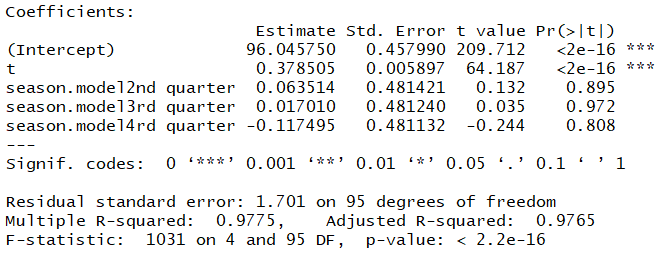
\includegraphics[width=0.7\textwidth]{summary_linearmodel}
    \caption{Summary statistics of the fitted linear model including check for seasonal components}
    \label{fig:summary_linearmodel}
\end{figure}

\begin{figure}[H]
    \centering
    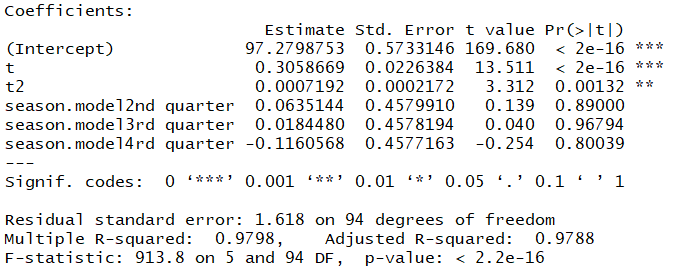
\includegraphics[width=0.7\textwidth]{summary_quadraticmodel}
    \caption{Summary statistics of the fitted quadratic model including check for seasonal components}
    \label{fig:summary_quadraticmodel}
\end{figure}

\begin{figure}[H]
    \centering
    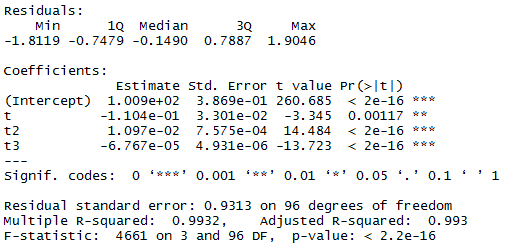
\includegraphics[width=0.7\textwidth]{summary_cubicmodel}
    \caption{Summary statistics of the fitted cubic model including check for seasonal components}
    \label{fig:summary_cubicmodel}
\end{figure}

\begin{figure}[H]
    \centering
    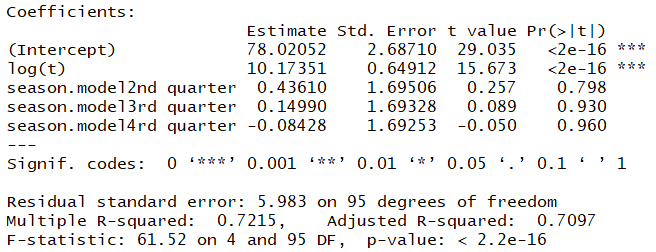
\includegraphics[width=0.7\textwidth]{summary_logmodel}
    \caption{Summary statistics of the fitted logarithmic model including check for seasonal components}
    \label{fig:summary_logmodel}
\end{figure}



\section{AICC-Matrix}
\label{sec:aicc_matrix}

\begin{figure}[H]
    \centering
    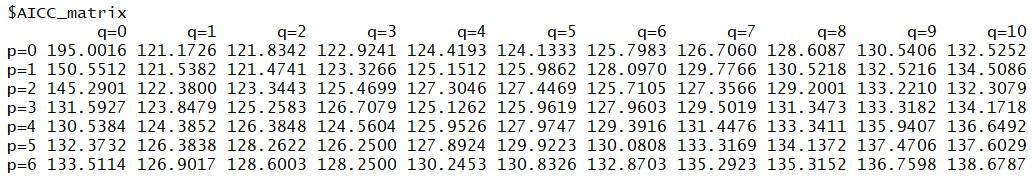
\includegraphics[width=0.7\textwidth]{aicc_matrix}
    \caption{AICC-Matrix (\citep{aic86})}
    \label{fig:aicc_matrix}
\end{figure}



\section{ACF/PACF-Plots of the unused polynomial Models}
\label{sec:ACFPACFunused}

\begin{figure}[H]
    \centering
    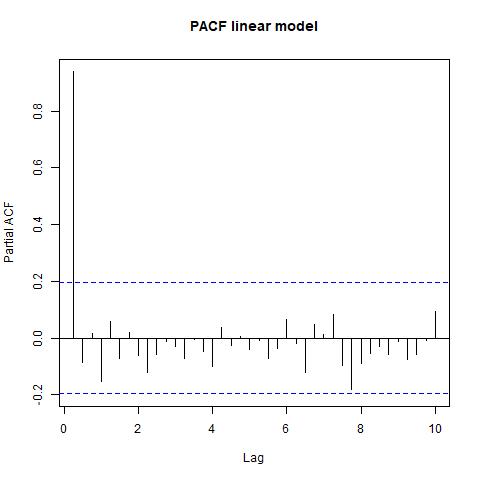
\includegraphics[width=0.6\textwidth]{acf_pacf_linearmodel}
    \caption{Sample Autocorrelation and Partial autocorrelation function of the linear model}
    \label{fig:acf_pacf_linearmodel}
\end{figure}

\begin{figure}[H]
    \centering
    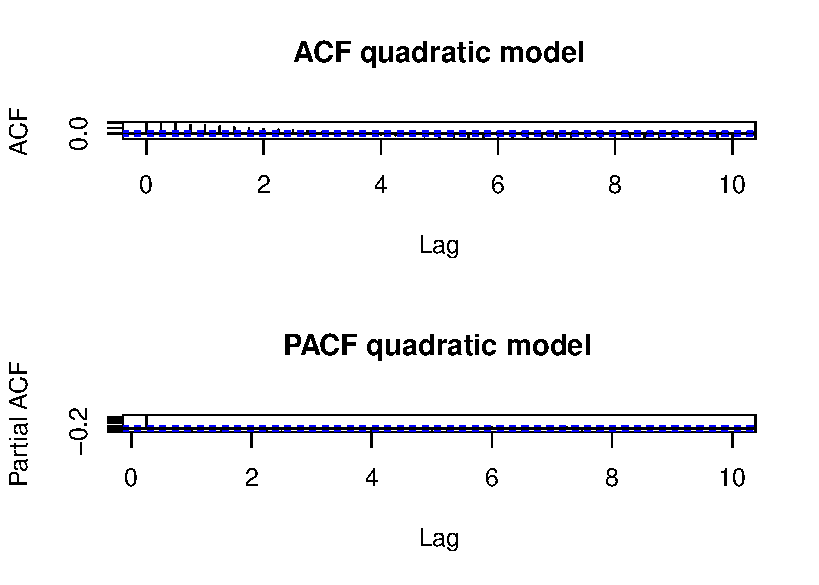
\includegraphics[width=0.6\textwidth]{acf_pacf_quadraticmodel}
    \caption{Sample Autocorrelation and Partial autocorrelation function of the quadratic model}
    \label{fig:acf_pacf_quadraticmodel}
\end{figure}

\begin{figure}[H]
    \centering
    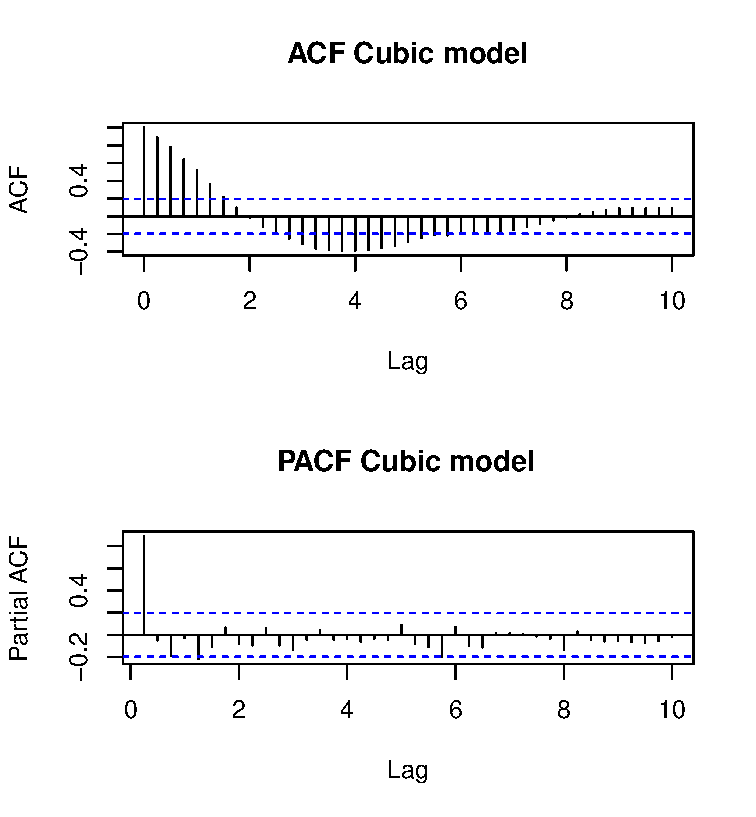
\includegraphics[width=0.7\textwidth]{acf_pacf_cubicmodel}
    \caption{Sample Autocorrelation and Partial autocorrelation function of the cubic model}
    \label{fig:acf_pacf_cubicmodel}
\end{figure}

\begin{figure}[H]
    \centering
    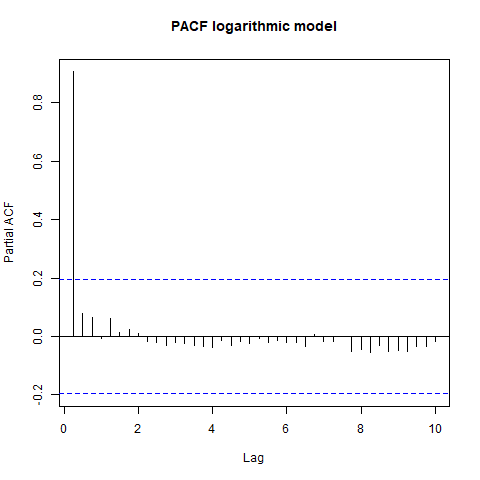
\includegraphics[width=0.7\textwidth]{acf_pacf_logmodel}
    \caption{Sample Autocorrelation and Partial autocorrelation function of the logarithmic model}
    \label{fig:acf_pacf_logmodel}
\end{figure}


% ------------------------------------------------------------------------


\section{Simulations of the model ACF/PACF}
\label{sec:simulations}

\begin{figure}[H]
    \centering
    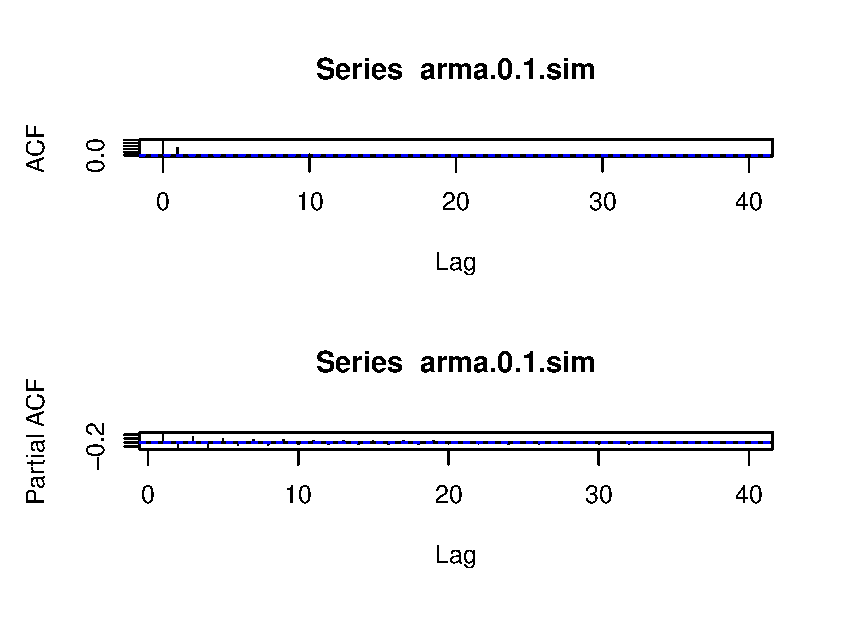
\includegraphics[width=0.7\textwidth]{sim_ma_1_00}
    \caption{Model ACF and PACF of a simulated MA(1)-process with $\theta_1 = 1.00$}
    \label{fig:sim_ma_1_00}
\end{figure}

\begin{figure}[H]
    \centering
    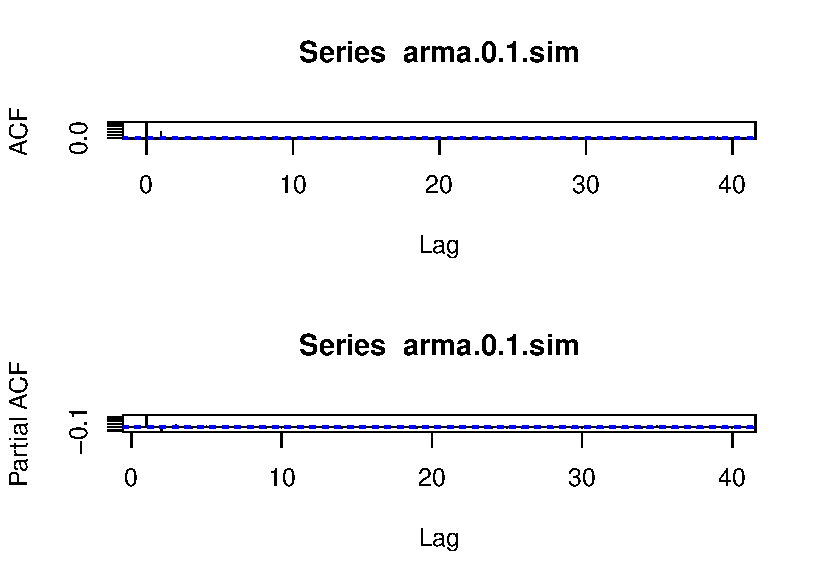
\includegraphics[width=0.7\textwidth]{sim_ma_1_05}
    \caption{Model ACF and PACF of a simulated MA(1)-process with $\theta_1 = 0.50$}
    \label{fig:sim_ma_1_05}
\end{figure}

\end{document}
